\chapter{Clasificación de Malware} \label{Capitulo_3}

Hoy en día, uno de los principales retos que enfrenta el software anti-malware es la enorme cantidad de datos y archivos que se requieren evaluar en busca de posibles amenazas maliciosas. Una de las razones principales de este volumen tan elevado de archivos diferentes es que los creadores de malware introducen variaciones en los componentes maliciosos para evadir la detección. Esto implica que los archivos maliciosos pertenecientes a la misma ``familia'' de malware (con patrones de comportamiento similares), se modifican constantemente utilizando diversas tácticas, lo que hace que parezcan ser múltiples archivos distintos \citep{kagglebig2015}. 


Para poder analizar y clasificar eficazmente estas cantidades masivas de archivos, es necesario agruparlos e identificar sus respectivas familias. Además, estos criterios de agrupación pueden aplicarse a nuevos archivos encontrados en computadoras para detectarlos como maliciosos y asociarlos a una familia específica. 


Para enfrentar este tipo de problema, se va a escoger una de las bases de datos disponibles en \citep{podder2021artificial} para poder clasificar distintos tipos de ciberataques. Como el objetivo principal de este trabajo es el estudio y puesta en práctica de diferentes algoritmos de aprendizaje automático, se ha decidido tomar como base de datos Microsoft Malware Classification Challenge. La principal razón de esta decisión ha sido que con este dataset tenemos a nuestra disposición dos algoritmos diferentes de machine learning que están referenciacios en este review y que se aborda el problema usando cada uno su propio enfoque. 



\section{Microsoft Malware Classification Challenge}



El conjunto de datos utilizado en este estudio proviene del Microsoft Malware Classification Challenge (BIG 2015) \citep{kagglebig2015}, una competición dirigida a la comunidad científica con el objetivo de promover el desarrollo de técnicas efectivas para agrupar diferentes variantes de malware. Se decidió escoger este dataset porque el objetivo que tengo en este trabajo es el de aprender y desarrollar diferentes métodos de aprendizaje automático y este dataset nos permite utilizar tanto una \acrshort{cnn} como un Autoencoder según \citep{podder2021artificial}. 

Se puede descargar desde su página web \citep{kagglebig2015}. Tiene un tamaño de 0.5 TB sin comprimir. Para poder manipularla en mi ordenador, tuve que seguir los siguientes pasos. Primero, me descargué la carpeta comprimida (7z) con todo el dataset. Después, la subí al servidor Simba de la facultad de informática y finalmente, usando el comando \textit{7zz x file\_ name.7z}, la descomprimí. 


Este dataset contiene 5 archivos:
\begin{itemize}
\item dataSample.7z - Carpeta comprida(7z) con una muestra de los datos disponibles.
\item train.7z - Carpeta comprida(7z) con los datos para el conjunto de entrenamiento.
\item trainLabels.csv - Archivo csv con las etiquetas asociadas a cada archivo de train.
\item test.7z - Carpeta comprida 7z con los datos sin procesar para el conjunto de prueba.
\item sampleSubmission.csv - Archivo csv con el formato de envío válido de las soluciones.
\end{itemize}



Para nuestro estudio, nos enfocaremos exclusivamente en el conjunto de datos de entrenamiento, que consta de los archivos ``train.7z'' y ``trainLabels.csv''. Los archivos 'test.7z' y 'sampleSubmission.csv' están destinados específicamente para la competición. Nosotros no los utilizaremos debido a que son programas de malware sin etiquetar y para este problema de clasificación, es necesario conocerlas.  Además, la carpeta 'dataSample.7z' proporciona dos programas que se encuentran también en la carpeta train.7z, por lo que tampoco la utilizaremos. 


Cada programa malicioso tiene un identificador, un valor hash de 20 caracteres que identifica de forma única el archivo, y una etiqueta de clase, que es un número entero que representa una de las 9 familias de malware al que puede pertenecer. Por ejemplo, el programa \textit{0ACDbR5M3ZhBJajygTuf} tiene como etiqueta el valor 7. Esta información se puede consultar en el archivo ``trainLabels.csv''. Cada programa tiene dos archivos, uno asm con el código extraído por la herramienta de desensamblado IDA y otro bytes\footnote{Realmente no es un archivo bytes, sino un fichero de texto con caractéres.} con la representación hexadecimal del contenido binario del programa pero sin los encabezados ejecutables (para garantizar esterilidad). Para nuestro estudio vamos a utilizar únicamente este ultimo archivo. 

\begin{figure}[h]
    \begin{center}
    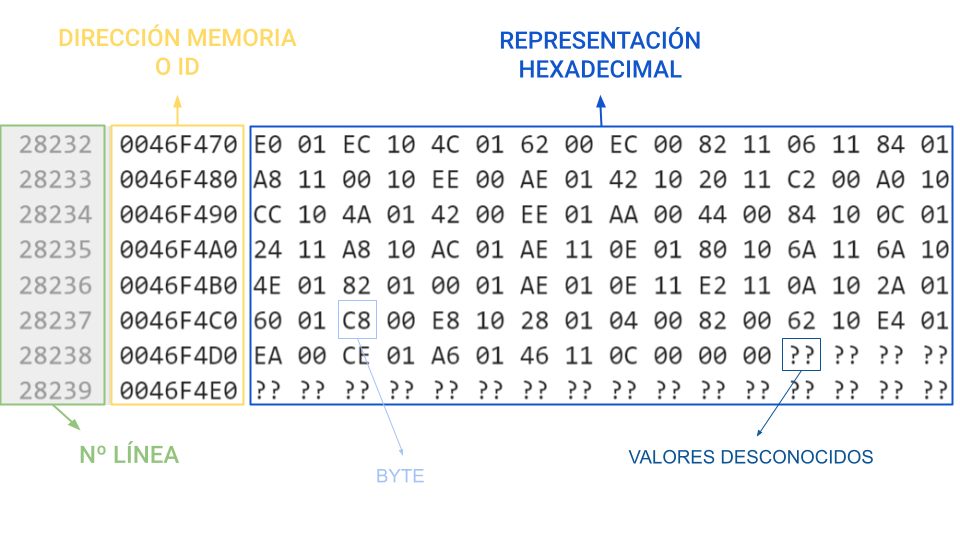
\includegraphics[width=0.7\textwidth]{img/previewMMC.png}
    \end{center}
    \caption{Explicación del contenido de ``0ACDbR5M3ZhBJajygTuf.bytes''.}
    \label{fig:previewMMC}
\end{figure} 


Como aparece en la figura \ref{fig:previewMMC}, los ocho primeros caracteres son direcciones de memoria, seguido de la representación hexadecimal del contenido binario del programa, que contiene 16 bytes (cada uno dos caracteres). A veces nos podemos encontrar con ``??'' en el lugar de un byte. Este símbolo se utiliza en estos archivos para representar que se desconoce su información porque su memoria no se puede leer \citep{cahyani2022influence}. 


\subsection{Distribución del dataset}

Hay un total de 21.741 programas de malware, pero nosotros tan solo usaremos los 10.868 pertenecientes al entrenamiento. Estos programas pertenecen a una de estas 9 familias de malware: Rammit, Lollipop, Kelihos\_ ver3, Vundo, Simda, Tracur, Kelihos\_ ver1, Obfuscator y Gatak. Según \cite{hu2019machine}, podemos deinirlas como: 

  

\begin{enumerate}

\item \textbf{Ramnit} es un malware tipo gusano que infecta archivos ejecutables de Windows, archivos de Microsoft Office y archivos HTML. Cuando se infectan, el ordenador pasa a formar parte de una red de bots controladas por un nodo central de forma remota. Este malware puede robar información y propagarse a través de conexiones de red y unidades extraíbles.

\end{enumerate}


\begin{wrapfigure}{l}{0.33\textwidth}
  \begin{center}
    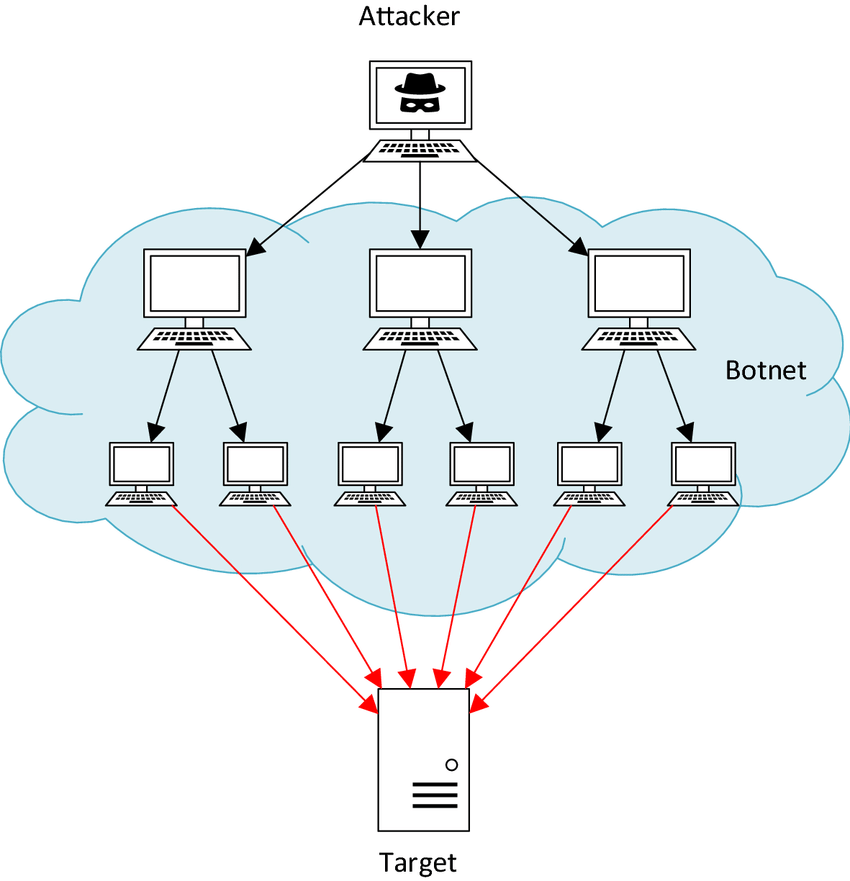
\includegraphics[width=0.33\textwidth]{img/botnetStructure.png}
  \end{center}
    \caption{Estructura de un botnet. Imagen sacada de \citep{botnetstructure}.}
  \label{fig:botnetstructure}
\end{wrapfigure}
\vspace{-\baselineskip}

\bigskip
\textbf{2.} \textbf{Lollipop} es un tipo de programa adware\footnote{Es una variedad de malware que muestra anuncios no deseados a los usuarios, típicamente como ventanas emergentes o banners.} que muestra anuncios no deseados en los navegadores web. También puede redirigir los resultados de búsqueda a recursos web ilegítimos, descargar aplicaciones maliciosas y robar la información del ordenador monitoreando sus actividades web. Este adware se puede descargar desde el sitio web del programa o empaquetarse con algunos programas de terceros.


\textbf{3.} \textbf{Simda} es un troyano backdoor\footnote{Un backdoor permite que una entidad no autorizada tome el control completo del sistema de una víctima sin su consentimiento.} que infecta ordenadores descargando y ejecutando archivos arbitrarios que pueden incluir malware adicional. Los ordenadores infectados pasar a ser parte de una botnet, lo que les permite cometer aciones criminales como robo de contraseñas, credenciales bancarias o descargar otros tipos de malware.

\textbf{4.} \textbf{Vundo} es otro troyano conocido por causar publicidad emergente para programas de antivirus falsos. A menudo se distribuye como un archivo DLL(Dynamic Link Library) \footnote{Una parte del programa que se ejecuta cuando una aplicación se lo pide. Se suele guardar en un directorio del sistema.} y se instala en el ordenador como un Objeto Auxiliar del Navegador (BHO) sin su consentimiento. Además, utiliza técnicas

\begin{enumerate}
\item[] avanzadas para evitar su detección y eliminación.
\item[5.] \textbf{Kelihos\_ ver3} es un troyano tipo backdoor que distribuye correos electrónicos que pueden contener enlaces falsos a instaladores de malware. Consta de tres tipos de bots \citep{kerkers2014characterisation}: controladores (operados por los dueños y donde se crean las instrucciones), enrutadores (redistribuyen las instrucciones a otros bots) y trabajadores (ejecutan las instrucciones).

\item[6.] \textbf{Tracur} es un descargador troyano que agrega el proceso 'explorer.exe' a la lista de excepciones del Firewall de Windows para disminuir deliberadamente la seguridad del sistema y permitir la comunicación no autorizada a través del firewall. Además, esta familia también te puede redirigir a enlaces maliciosos para descargar e instalar otros tipos de malware.

\item[7.] \textbf{Kelihos\_ ver1} es una versión más antigua del troyano Kelihos\_ ver3, pero con las mismas funcionalidades.

\item[8.] \textbf{Obfuscator.ACY} es un tipo de malware sofisticado que oculta su propósito y podría sobrepasar las capas de seguridad del software.  Se puede propagar mediante archivos adjuntos de correo electrónico, anuncios web y descargas de archivos. 
\item[9.] \textbf{Gatak} es un troyano que abre una puerta trasera en el ordenador. Se propaga a través de sitios web falsos que ofrecen claves de licencias de productos. Una vez infectado el sistema, Gatak recopila información del ordenador.
\end{enumerate} 

Como ya mencionamos antes, vamos a entrenar nuestras redes neuronales con 10.868 archivos bytes. De estos archivos, solo son válidos 10.860 porque en los 8 archivos restantes\footnote{Los identificadores de estos archivos son 58kxhXouHzFd4g3rmInB, 6tfw0xSL2FNHOCJBdlaA, a9oIzfw03ED4lTBCt52Y, cf4nzsoCmudt1kwleOTI, d0iHC6ANYGon7myPFzBe, da3XhOZzQEbKVtLgMYWv, fRLS3aKkijp4GH0Ds6Pv, IidxQvXrlBkWPZAfcqKT.} (pertenecientes a la familia Ramnit), todo sus bytes son ``??''. Con estos datos finales, vamos a ver gráficamente como se distribuyen las 9 clases de malware (Figura \ref{img: circularMMC}).

\begin{figure}[h]
    \begin{center}
    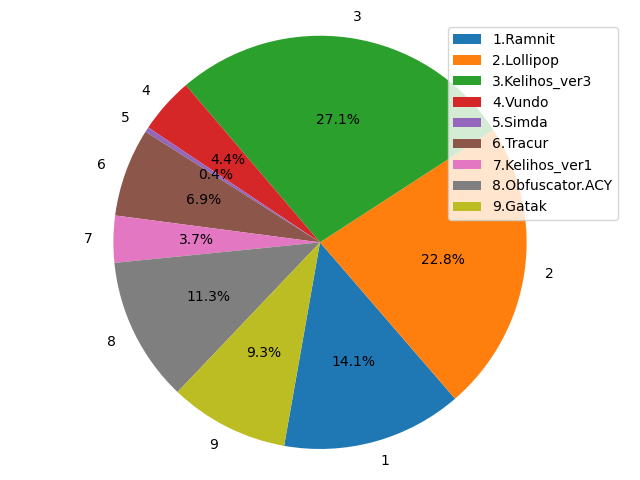
\includegraphics[width=0.6\textwidth]{img/circularMMC.png}
    \end{center}
    \caption{Distribución del BIG 2015 training dataset.}
    \label{img: circularMMC}
\end{figure}  

Analizando la Figura \ref{img: circularMMC}, podemos observar como la distribución entre las clases no es uniforme. Mientras que de la clase Simbda hay 42 muestras, de la clase Kelihos\_ ver3 hay 2.942, es decir, 70 veces más de muestras. En \citep{kebede2017classification} deciden prescindir de esta clase, pero nosotros hemos decidido hacer el análisis con las 9 clases. 


A la hora de crear nuestros modelos, hemos dividido el conjunto de datos aleatoriamente usando la función \texttt{train\_test\_split()} en grupos del 75\%, 15\% y 10\% para entrenamiento, test y validación respectivamente. La tabla \ref{tab:malware_distribution} muestra como quedarían distribuidas las clases en los diferentes grupos.

\begin{table}[h]
\centering
\begin{tabular}{lccccccccc}
\hline
& Ramnit & Lollipop & Kelihos3 & Vundo & Simda & Tracur & Kelihos1 & Obfus & Gatak \\
\hline
Total & 1533 & 2478 & 2942 & 475 & 42 & 751 & 398 & 1228 & 1013 \\
Train & 1177 & 1835 & 2228 & 337 & 26 & 543 & 306 & 925 & 768 \\
Test & 223 & 394 & 436 & 75 & 9 & 124 & 42 & 177 & 149 \\
Valid & 133 & 249 & 278 & 63 & 7 & 84 & 50 & 126 & 96 \\
\hline
\end{tabular}
\caption{Distribución de los tipos de malware en los conjuntos de datos}
\label{tab:malware_distribution}
\end{table}

 


Para abordar este problema de clasificación, vamos a realizar dos modelos diferentes para luego comparar sus resultados. El primer método de machine learning que vamos a utilizar es una \acrfull{cnn}. El segundo será entrenar un Autoencoder junto con una \acrfull{dnn}, primero obteniendo una representación comprimida de los datos y después clasificando esta representación con una red neuronal profunda. 
 







\section{Red Neuronal Convolucional}

10800 archivos de prueba de tipo .bytes (otros 10800 de tipo .asm) pero solo usaremos los .bytes. Convertimos cada archivo en una imagen. Primero, cada código hexadecimal lo convertimos a numeros decimales y estos los pasamos a un array de numpy. Hacemos reshape (lado,lado2) de forma que obtengamos la mayor dimension posible que sea casi cuadrado consiguiendo perder la menor información posible. Este reshape lo pasamos a np.uint8 y finalmente lo interpolamos usando bilinal, cubic, bicubic, nearest y observamos cual es la mejor de todas {zhao2023new} (hacer una grafica o algo para comprobarlo). Además, para caragr los datos he usado multiprocessing con los diferentes datos de tiempo. En el caso de algunas imagenes, los archivos .bytes no contienen ningun tipo de informacion(?? ?? ?? ..) todos los byte son ??. Estos ficheros, no estan incluidos en las imagenes ni de entrenamiento ni validación porque no contienen ningun tpo de información. 

La diferencia principal entre realizar el entrenamiento del modelo en la GPU o en la CPU radica en el rendimiento y la velocidad de entrenamiento.

\subsection{GPU (Unidad de Procesamiento Gráfico)}

\subsubsection{Ventajas}
\begin{itemize}
    \item Las GPU están diseñadas específicamente para manejar operaciones matriciales y paralelas, que son comunes en el entrenamiento de modelos de redes neuronales.
    \item Pueden realizar cálculos en paralelo en grandes cantidades de datos, lo que acelera significativamente el entrenamiento de modelos, especialmente en tareas intensivas en cálculos, como las redes neuronales profundas.
    \item Ofrecen un rendimiento superior en comparación con las CPU para tareas de aprendizaje profundo.
\end{itemize}

\subsubsection{Desventajas}
\begin{itemize}
    \item Pueden ser más costosas y consumir más energía que las CPU.
    \item Puede haber limitaciones en la cantidad de memoria de la GPU disponible, lo que podría ser un factor en modelos muy grandes.
\end{itemize}

\subsection{CPU (Unidad Central de Procesamiento)}

\subsubsection{Ventajas}
\begin{itemize}
    \item Disponibles en la mayoría de las computadoras y servidores sin necesidad de hardware adicional.
    \item Adecuadas para tareas generales de propósito múltiple y no solo para aprendizaje profundo.
    \item Pueden ser más económicas en términos de hardware y consumo de energía.
\end{itemize}

\subsubsection{Desventajas}
\begin{itemize}
    \item Las CPU no están diseñadas específicamente para tareas de aprendizaje profundo y pueden ser menos eficientes en términos de velocidad para ciertos tipos de operaciones, especialmente en modelos grandes.
\end{itemize}

\section{Autoencoder}
\section{Resultados}















\citep{gibert2022fusing} mete imagen de asm junto con bytes.
\begin{comment}

\begin{figure}[h]
    \begin{center}
    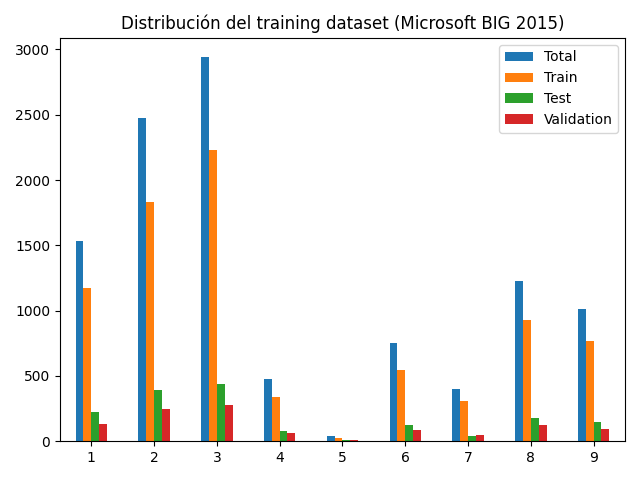
\includegraphics[width=0.6\textwidth]{img/barras4MMC.png}
    \end{center}
    \caption{Distribución de las clases en cada grupo.}
    \label{img: train_test_valMMC}
\end{figure}

\section{Resumen del Conjunto de Datos}

El conjunto de datos utilizado en este estudio proviene del Desafío de Clasificación de Malware de Microsoft (BIG 2015), accesible a través de Kaggle. Este conjunto de datos consta de programas de malware pertenecientes a 9 categorías diferentes. Se proporcionan conjuntos de datos de entrenamiento y prueba, pero solo se utilizan los datos de entrenamiento debido a la falta de etiquetas para el conjunto de prueba para su entrega. Además

El conjunto de entrenamiento contiene 10,868 muestras de malware, cada una con un identificador único, un valor hash de 20 caracteres y una etiqueta de clase que representa una de las 9 familias de malware. Cada archivo de malware tiene una representación hexadecimal de su contenido binario, junto con un archivo 'bytes' que contiene esta información. No se excluye ninguna categoría de malware en este estudio.

La distribución de los datos se realiza con un 72\% para entrenamiento, un 8\% para validación y un 20\% para pruebas. Se realizan varias divisiones y análisis de los conjuntos de datos para ajustar y evaluar diferentes modelos y enfoques de aprendizaje profundo para la clasificación de malware.

Este conjunto de datos, con su amplia gama de muestras etiquetadas y la diversidad de familias de malware representadas, proporciona una base sólida para la investigación y desarrollo de métodos efectivos de detección y clasificación de amenazas informáticas.













\item Worm (Gusano)- Los gusanos informáticos son un tipo de malware que puede propagarse a través de redes sin la intervención de un programa huésped o de un humano. Son caballos de Troya maliciosos que pueden replicarse y propagarse de una computadora a otra. Los gusanos infectan a sus anfitriones mediante el engaño y la astucia, pudiendo causar graves daños a las computadoras comprometidas al consumir ancho de banda, sobrecargar sistemas, eliminar o modificar archivos e instalar virus adicionales. Además, las vulnerabilidades en el software, los archivos adjuntos de correo electrónico y las conexiones de red pueden facilitar su propagación. 

\item Adware (programa publicitario) - El adware es una variedad de malware que muestra anuncios no deseados a los usuarios, típicamente como ventanas emergentes o banners. A menudo se distribuye como parte de descargas de software gratuitas, pero también se puede obtener a través de un ciberataque o una vulnerabilidad. El adware tiene como objetivo generar ingresos para sus desarrolladores mostrando anuncios a los consumidores. Sin embargo, puede causar un daño significativo a una computadora infectada al degradar su rendimiento, reducir su disponibilidad y violar la privacidad del usuario al recopilar información sobre sus actividades de navegación.

\item Backdoor (Puerta trasera) - Un backdoor permite que una entidad no autorizada tome el control completo del sistema de una víctima sin su consentimiento. Un troyano de puerta trasera siempre se presenta como una herramienta de software legítima esencialmente requerida por el usuario. Otras opciones pueden ser visitar un sitio web malicioso o hacer clic en un enlace no deseado. Al ejecutarse, se añade a sí mismo en la rutina de inicio del sistema y busca una conexión a Internet. Una vez que el sistema está en línea, se conecta con su autor, quien luego toma el control del sistema para realizar diferentes tareas, como descargar/cargar archivos, registrar pulsaciones de teclas, enviar correos electrónicos no deseados o robar contraseñas, entre otras cosas.

\item Trojan (Troyano)- Los troyanos son programas maliciosos que se disfrazan como programas o archivos legítimos y pueden tomar el control de una computadora para ejecutar operaciones maliciosas como robar datos, dañar el sistema o abrir puertas traseras para otros virus. El término "Troyano" proviene de la leyenda griega del caballo de Troya, una táctica engañosa utilizada para conquistar Troya. En el ámbito digital, los troyanos son parásitos digitales hostiles capaces de leer contraseñas, grabar pulsaciones de teclas y propagar otros virus. Se utilizan técnicas de ingeniería social, como correos electrónicos de phishing o descargas maliciosas, para propagarlos. A diferencia de los virus informáticos y los gusanos, los troyanos no pueden replicarse y deben ser instalados o ejecutados por los usuarios.

\item Trojan downloader (Descargador troyano) - Es un programa malicioso que se descarga e instala en una computadora infectada. Puede abrir conexiones de red ilícitas, mutarse a sí mismo, deshabilitar herramientas de seguridad y transferir información personal del usuario sin permiso. Además, su función principal es la de descargar e instalar otro malware dañino en el sistema infectado.

\item Obfuscated malaware (Malware obfuscado) - La obfuscación es una técnica utilizada para hacer que el código de un programa sea más difícil de entender o de analizar. Esto implica modificar el código del programa malicioso de manera que sea más complicado para los investigadores de seguridad o los programas antivirus detectarlo y comprender cómo funciona. Su objetivo principal es eludir la detección y análisis por parte de los programas antivirus y otros sistemas de seguridad.













\item Ramnit es un malware de tipo gusano detectado en el 2011 y que afecta sistemas operativos Windows. , pueden ser utilizadas para múltiples objetivos maliciosos. Ramnit es una avanzada herramienta para criminales con funcionalidades de rootkit, no detección por antivirus, inyección Web y uso de comunicaciones cifradas con el centro de Comando y Control. Ramnit es un malware que ha sido utilizado para realizar actividades criminales, entre las que se pueden destacar. Monitorización de la navegación web del sistema infectado y detectar la visita de sitios de banca online. Manipulación de webs de banca online con el objetivo de parecer legitimar. Robo de cookies de sesión de los navegadores web para poder suplantar a la víctima en sitios seguros. Escaneo los discos duros de la computadora y robo archivos en base a palabras clave (como contraseñas). Acceso de forma remota a los ordenadores afectados. Recopilación de las credenciales de acceso de clientes de FTP.
¿Cómo me infecta? Se cree que su propagación es través de enlaces de confianza enviados a través de correos electrónicos de phishing o mediante redes sociales, que están principalmente orientados principalmente al robo de dinero de cuentas bancarias de victimas con sistemas operativos Windows. También se ha detectado el uso servidores FTP públicos para la distribución del malware.


\item Lollipop (L) is an adware that produces profits for the developer by automatically showing advertisements on the user
computer.
\item 1 Swizzor Swizzor is a type of malware flies that under the radar to deliver unsolicited advertisements, modifying browser setting without
user permission.
2 Vundo Vundo is either a Trojan horse or a computer worm that is known to cause Pop-up advertising for rogue antispyware programs.
3 Spybot Spybot is a type of worm that usually arrives on a computer through peer-to-peer file sharing, specifically through the Kazaa file
sharing network. Its many variants sometimes have other ways of spreading.
4 Ransom Ransom is a type of malware that can be covertly installed on a computer without knowledge or intention of the user that
restricts access to the infected computer system in some way, and demands that the user pay a ransom to the malware
operators to remove the restriction.
5 Ramnit Ramnit is a type of virus that infects Windows executable files and HTML files. It can also give a malicious hacker access to
your computer. It spreads through infected removable drives, such as USB flash drives.
6 Lollipop Lollipop is a type of adware program that shows advertisements as you browse the web. It can also redirect your search engine
results, monitor what you do on your computer, download applications, and send information about your computer to a hacker.
7 Kelihos Kelihos is a type of trojan that can give a malicious hacker access and control of your computer. The family spreads by sending
spam emails that have links to other malware.
8 Delf Delf is a type of trojan that reports and intercepts Internet traffic and may also download unwanted applications onto your
computer.
9 Banker Banker is a type of data-stealing trojans that can capture your online banking details, such as your log 

\citep{tang2019dynamic}

\item Simda es un malware de tipo troyano que infecta ordenadores con sistema operativo Windows. Los ordenadores infectados con este malware pasan a ser parte de una botnet, con lo que pueden ser utilizados para cometer acciones criminales o maliciosas.

¿Qué hace?	
Esta familia de malware incluye funcionalidades de backdoor, robo de contraseñas, robo de credenciales bancarias y es capaz de descargar otro tipo de malware.

Sistemas afectados	
Principalmente sistemas Windows:

Windows XP
Windows Vista
Windows 7
Windows 8
¿Cómo me infecta?	
El contagio de esta amenaza es mediante la distribución de archivos previamente infectados o a través de redes compartidas.

\item Obfuscation malware, also known as obfuscation techniques or code obfuscation, is a strategy employed by cybercriminals to hide the true intent and functionality of their malicious code. Essentially, it’s a way of making malware more difficult to detect and analyze by security software and researchers.

Compression, encryption, and encoding are some of the most common obfuscation methods used by threat actors. Multiple methods are often used in tandem to evade a wider variety of cyber security tools at the initial point of intrusion.

\item Gatak is a backdoor trojan that first appeared in 2012. Another name for this threat is Stegoloader, and its main distinctive feature is its ability to communicate with its C&C servers via steganography.

El grupo detrás de Trojan Gatak (Trojan.Gatak) continúa siendo una amenaza para las compañías, especialmente para el sector salud, fuertemente impactado por los ataques. Gatak es conocido por infectar a sus víctimas por medio de sitios web que prometen claves de licencias de producto para software pirata. Si bien el grupo se enfocó inicialmente en blancos en los Estados Unidos, a lo largo de los últimos dos años se ha diversificado y los ataques se llevan a cabo ahora contra compañías en varios países.

La mayor parte de las infecciones de Gatak (62%) ocurre en computadoras corporativas. El análisis de recientes ataques corporativos indica que el sector de la salud es, sin lugar a dudas, el más impactado por Gatak. De las 20 principales compañías más afectadas (compañías con más computadoras infectadas), 40% eran en el sector de la salud. En el pasado, el sector de seguros también quedó fuertemente en la mira del grupo.

Sitio web de generación de claves para licencias usado para atraer a las víctimas inocentesLas víctimas de Gatak son infectadas usando sitios web que ofrecen generar claves para licencias de productos o "keygens" de software pirata. El malware es empaquetado con la clave del producto y, si la víctima es inducida a bajar y abrir uno de esos archivos, el malware se instala clandestinamente en su computadora.

Los responsables del ataque parecen enfocarse en ofrecer claves de producto para softwares que son más probables que se utilicen en entornos profesionales. Los sitios web usados ​​en los ataques son controlados por los grupos de ataque y no tienen relación con los desarrolladores del software. En ningún momento se comprometen las versiones legítimas del software. Entre las marcas de softwares usadas ​​como anzuelos se han identificado:
SketchList3D (software de diseño para carpintería)
Native Instruments Drumlab (software de ingeniería de audio)
BobCAD-CAM (software de manufactura/metalúrgica)
BarTender Enterprise Automation (software de creación de etiquetas y código de barras)
HDClone (utilitario de clonaje de disco rígido)
Siemans SIMATIC STEP 7 (software de automación industrial)
CadSoft Eagle Professional (software de diseño de placa de circuito impreso)
PremiumSoft Navicat Premium (software de administración de base de datos)
Originlab Originpro (software gráfico para análisis de datos)
Manctl Skanect (software de digitalización 3D)
Symantec System Recovery (software de backup y recuperación de datos; ahora parte de Veritas)
Las claves de producto bajadas a partir de estos sitios no funcionan y simplemente generan una secuencia pseudoaleatoria de caracteres. Eso significa que todo lo que la víctima recibe con la descarga es un archivo inútil y una posible infección de Gatak.
Herramientas de Malware
Trojan Gatak (también conocido por Stegoloader) ha sido utilizado en ataques por lo menos desde 2011. Existen dos componentes principales de malware. Un módulo de implementación leve (Trojan.Gatak.B) puede realizar una identificación detallada del sistema en las computadoras infectadas e instalar selectivamente cargas adicionales. El módulo principal (Trojan.Gatak) es un verdadero Troyano de backdoor, que mantiene una presencia persistente en una computadora infectada y roba su información.

Una característica notable de Gatak es el uso de esteganografía, una técnica que esconde datos dentro de archivos de imagen. Cuando Gatak se instala en una computadora, intenta bajar un archivo de imagen PNG de una serie de direcciones URL codificadas en el malware. La imagen se parece a una fotografía común, sin embargo, contiene un mensaje cifrado dentro de sus datos de pixel. Trojan Gatak es capaz de decodificar este mensaje, que contiene comandos y archivos para su ejecución.
En casi el 62% de los incidentes, el movimiento lateral en la red de la víctima se produce dentro de las dos horas tras la infección. En los casos restantes, el movimiento lateral se inició en algún momento después de dos horas. La variación indica que el movimiento lateral no es automático, sino que se ejecuta manualmente por los grupos de ataque. No se sabe con precisión si los grupos de ataque poseen los recursos para explorar todas las infecciones inmediatamente o si ellos priorizan algunas infecciones sobre otras.

Poco se sabe acerca de cómo los grupos de ataque se mueven en la red de una compañía. La explicación más probable es que ellos exploran contraseñas débiles y una seguridad pobre en archivos compartidos y en las unidades de red. No existe evidencia de ataques de día cero o que se empleen herramientas sofisticadas de hacking.

En algunos casos, los grupos de ataque infectaron computadoras con otros tipos de malware, incluso varias variantes de ransomware y el Troyano financiero Shylock (Trojan.Shylock). En el caso de Shylock, estas parecen ser versiones más antiguas de la amenaza y pueden incluso ser infecciones de "bandera falsa". Pueden utilizarse ​por el grupo cuando creen que su ataque fue descubierto, a fin de engañar a los investigadores.
¿Por qué el área de la salud?
Poco se sabe acerca del grupo responsable de Gatak, si bien la naturaleza corporativa de sus blancos, en conjunto con la ausencia de vulnerabilidades de día cero o módulos de malware avanzados, sugieren que pueden ser cibercriminales en su esencia, aunque también existen recursos dentro del malware para operaciones más tradicionales de espionaje.

No está claro como Gatak está obteniendo lucro con sus ataques. Una posibilidad es el robo de datos, con los grupos de ataque vendiendo información de identificación personal y otros datos robados en el cibermercado clandestino. Esto podría explicar el foco determinado de los grupos de ataque en el sector de la salud, pues los registros con información de salud normalmente se venden a mejores precios comparados con otra información personal.

Sin embargo, los medios de distribución de Gatak, a través de sitios de generación de claves de licencia, indican que los grupos de ataque pueden ser más oportunistas. Al utilizar un abordaje watering-hole, los grupos de ataque desempeñan un papel en gran parte pasivo, con relativamente poco control sobre quien es infectado. Si este es el caso, el sector de la salud puede simplemente ser el más susceptible a este tipo de ataque.

Las compañías de salud muchas veces pueden estar bajo presión, con pocos recursos, y muchas usan sistemas de software legados cuyas actualizaciones son muy caras. Por consiguiente, los profesionales podrían ser más propensos a tomar atajos e instalar software pirata. Si bien parece que las compañías de otros sectores se infectan con menos frecuencia, los grupos de ataque no parecen ignorar o remover esas infecciones cuando se producen.





















un conjunto de datos de malware sin precedentes y promoviendo el desarrollo de técnicas efectivas de código abierto para agrupar variantes de archivos de malware en sus respectivas familias.

Est Fue un challenge que promocionó Microsoft para que la comunidad científica propuesiera una solución para este problema.Es un dataset que fue creado para un Challenge proporcionado por Microsoft para 
Dataset Description
Warning: this dataset is almost half a terabyte uncompressed! We have compressed the data using 7zip to achieve the smallest file size possible. Note that the rules do not allow sharing of the data outside of Kaggle, including bit torrent (why not?).

You are provided with a set of known malware files representing a mix of 9 different families. Each malware file has an Id, a 20 character hash value uniquely identifying the file, and a Class, an integer representing one of 9 family names to which the malware may belong:

Ramnit
Lollipop
Kelihos_ver3
Vundo
Simda
Tracur
Kelihos_ver1
Obfuscator.ACY
Gatak
For each file, the raw data contains the hexadecimal representation of the file's binary content, without the PE header (to ensure sterility).  You are also provided a metadata manifest, which is a log containing various metadata information extracted from the binary, such as function calls, strings, etc. This was generated using the IDA disassembler tool. Your task is to develop the best mechanism for classifying files in the test set into their respective family affiliations.

The dataset contains the following files:

train.7z - the raw data for the training set (MD5 hash = 4fedb0899fc2210a6c843889a70952ed)
trainLabels.csv - the class labels associated with the training set
test.7z - the raw data for the test set (MD5 hash = 84b6fbfb9df3c461ed2cbbfa371ffb43)
sampleSubmission.csv - a file showing the valid submission format
dataSample.csv - a sample of the dataset to preview before downloading

dropout25
Model: "sequential_2"
_________________________________________________________________
 Layer (type)                Output Shape              Param #   
=================================================================
 conv2d_26 (Conv2D)          (None, 224, 224, 64)      1792      
                                                                 
 conv2d_27 (Conv2D)          (None, 224, 224, 64)      36928     
                                                                 
 max_pooling2d_10 (MaxPooli  (None, 112, 112, 64)      0         
 ng2D)                                                           
                                                                 
 conv2d_28 (Conv2D)          (None, 112, 112, 128)     73856     
                                                                 
 conv2d_29 (Conv2D)          (None, 112, 112, 128)     147584    
                                                                 
 max_pooling2d_11 (MaxPooli  (None, 56, 56, 128)       0         
 ng2D)                                                           
                                                                 
 conv2d_30 (Conv2D)          (None, 56, 56, 256)       295168    
                                                                 
 conv2d_31 (Conv2D)          (None, 56, 56, 256)       590080    
                                                                 
 conv2d_32 (Conv2D)          (None, 56, 56, 256)       590080    
                                                                 
 max_pooling2d_12 (MaxPooli  (None, 28, 28, 256)       0         
 ng2D)                                                           
                                                                 
 conv2d_33 (Conv2D)          (None, 28, 28, 512)       1180160   
                                                                 
 conv2d_34 (Conv2D)          (None, 28, 28, 512)       2359808   
                                                                 
 conv2d_35 (Conv2D)          (None, 28, 28, 512)       2359808   
                                                                 
 max_pooling2d_13 (MaxPooli  (None, 14, 14, 512)       0         
 ng2D)                                                           
                                                                 
 conv2d_36 (Conv2D)          (None, 14, 14, 512)       2359808   
                                                                 
 conv2d_37 (Conv2D)          (None, 14, 14, 512)       2359808   
                                                                 
 conv2d_38 (Conv2D)          (None, 14, 14, 512)       2359808   
                                                                 
 max_pooling2d_14 (MaxPooli  (None, 7, 7, 512)         0         
 ng2D)                                                           
                                                                 
 flatten_2 (Flatten)         (None, 25088)             0         
                                                                 
 dense_6 (Dense)             (None, 4096)              102764544 
                                                                 
 dropout_2 (Dropout)         (None, 4096)              0         
                                                                 
 dense_7 (Dense)             (None, 4096)              16781312  
                                                                 
 dropout_3 (Dropout)         (None, 4096)              0         
                                                                 
 dense_8 (Dense)             (None, 9)                 36873     
                                                                 
=================================================================
Total params: 134297417 (512.30 MB)
Trainable params: 134297417 (512.30 MB)
Non-trainable params: 0 (0.00 Byte)
_________________________________________________________________
\end{comment}




